\subsection{Interrupts}
A key concept in embedded systems is the need to process external stimuli,
like a button press, or when a sensor detects a change in its environment.
However, the microcontroller may already be busy executing another long
running task - maybe it's waiting on a second sensor, or its busy updating
a large display. The most efficient way to handle this issue is with
\emph{interrupts}.

An interrupt is a signal that is generated by the hardware or software
when an event occurs that needs immediate attention. Once it's fired
from an interrupt source, say a rising edge on a GPIO pin, the
interrupt signal arrives at the CPU, which - if the conditions are right
and the correct bits are set - saves what it's doing, and executes a
special function called an interrupt service routine (ISR), also called
an interrupt handler.

An interrupt is a special type of exception. Others relevant to MCUs are
faults, traps, and resets. Peripherals can raise interrupts. The
CPU can be interrupted by more than one event, each of which has its own
ISR stored in the interrupt vector table. Interrupts can be enabled or
disabled. Interrupts may have different priorities, and higher priorities
can preempt lower priorities. This means that when the CPU is servicing
one interrupt, an interrupt with a higher priority can interrupt and make
the CPU service it instead.

The flow of an interrupt is thus:
\begin{enumerate}
    \item A peripheral raises an interrupt.
    \item The CPU checks if $N$ is enabled.
    \item If $N$ is enabled, the CPU marks $N$ as pending.
    \item The CPU checks the priority of $N$ versus the current
          priority level, as it might be serving a higher priority interrupt.
    \item If the priority of $N$ is greater than the current priority
          level, then the CPU updates the current priority level to the level of
          the new interrupt and pushes the CPU state to the stack.
          It then puts the $N$th entry in the vector table into the program
          counter, a special register that keeps track of where the CPU
          is in the code. The ISR is now running.
\end{enumerate}
\begin{figure}
    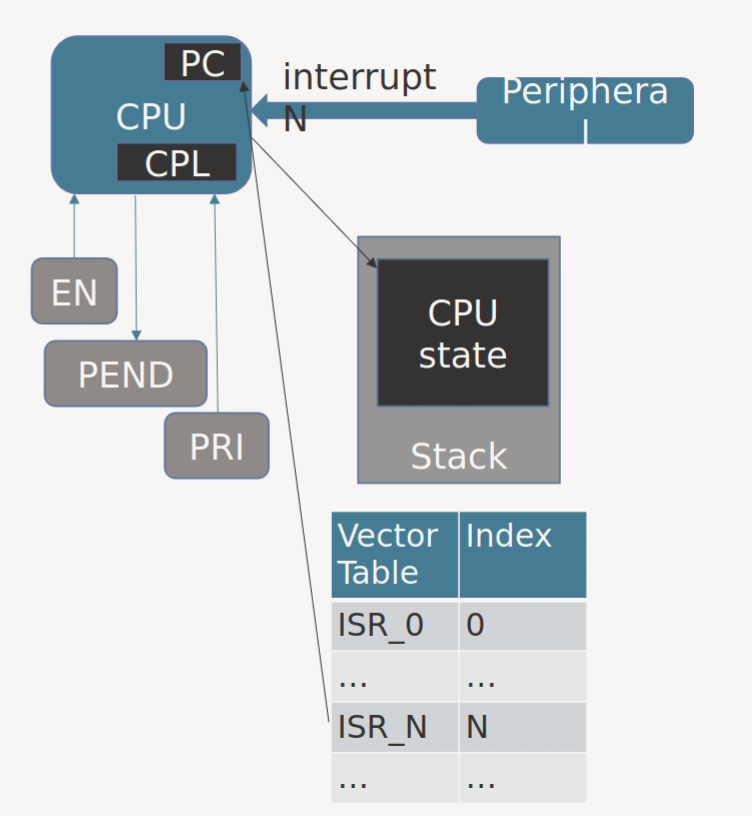
\includegraphics{images/interrupt_flow.png}
    \caption{Interrupt Flow}
    \label{fig:interrupt}
\end{figure}

\marginnote{A common exam question is "how many times was the interrupt handler interrupted?"
    or "how many times was the CPU state restored?".}

\subsection{Exceptions}
We mentioned several other types of exceptions. While interrupts are
usually handled at the end of instructions and the CPU resumes at the
next instruction, faults happen in the middle of an instruction and
execution resumes in the same instruction. Just as with interrupts,
higher-priority exceptions may preempt lower-priority exceptions.

On an ARM MCU, when an exception/interrupt is raised,
the NVIC decides things like
\begin{itemize}
    \item Is the exception enabled or should it be ignored?
    \item Is the interrupt above the current priority level?
    \item Is the interrupt already pending?
\end{itemize}
When an exception handler is invoked, the
current program stops running. The \texttt{r0}-\texttt{3},
\texttt{r12}, \texttt{LR}, \texttt{PC}, and \texttt{PSR}
are pushed onto the stack. These are the registers
that ABI allows you to modify. \texttt{LR} holds a
special value that is not the PC of the program.
The priority level is set to that of the current
invoked exception, and the ISR address is looked
up in the vector table. The program then branches
to that address by setting the PC to point there.

Other registers important to interrupts are the
\emph{bit reset register} (BRR) and
\emph{bit set and reset register} (BSRR).
For each \texttt{1} bit written to the lower 16
bits of BRR, the corresponding bit in the ODR
is turned off. For each \texttt{1} bit written
to the lower 16 bits of BSRR, the corresponding
bit in the ODR is turned on. For each \texttt{1}
bit written to the higher 16 bits of the BSRR,
the corresponding ODR bit is turned off.

A single write to BRR or BSRR is \emph{atomic}
in the sense that it will either happen or it
won't, as opposed to an operation that can be
interrupted halfway by something like another
thread or an interrupt.
